\clearpage
\section{Podstawa teoretyczna}
\label{sec:podstawa}


\subsection{Synchrotron}
	
	\hspace{2em} Synchrotron to urządzenie służące do nadawania cząstkom elementarnym (elektronom, protonom) bardzo wysokich energii za pomocą odpowiedniego układu zmiennych zsynchronizowanych pól elektrycznych i magnetycznych. W układzie tym pole elektryczne przyspieszając cząstkę przekazuje jej energię, a pole magnetyczne służy do utrzymania ruchu cząstki na torze stacjonarnym. 
	Synchrotron jest rodzajem akceleratora cząstek, w którym pole elektromagnetyczne zakrzywiające trajektorię wiązki cząstek jest synchronizowane z tą wiązką aby zwiększyć jej energię kinetyczną. W przeciwieństwie do innego rodzaju akceleratorów pole elektromagnetyczne nie jest stałe - zarówno siła jak i częstotliwość mogą się zmieniać w czasie. Pozwala to na uzyskanie ruchu po okręgu o stałym promieniu przez cały czas trwania procesu przyspieszania cząstek. Schemat synchrotronu przedstawiono na rys. (\ref{fig:schematSynchrotronu}).
	
	\begin{figure}[ht]
		\centering
		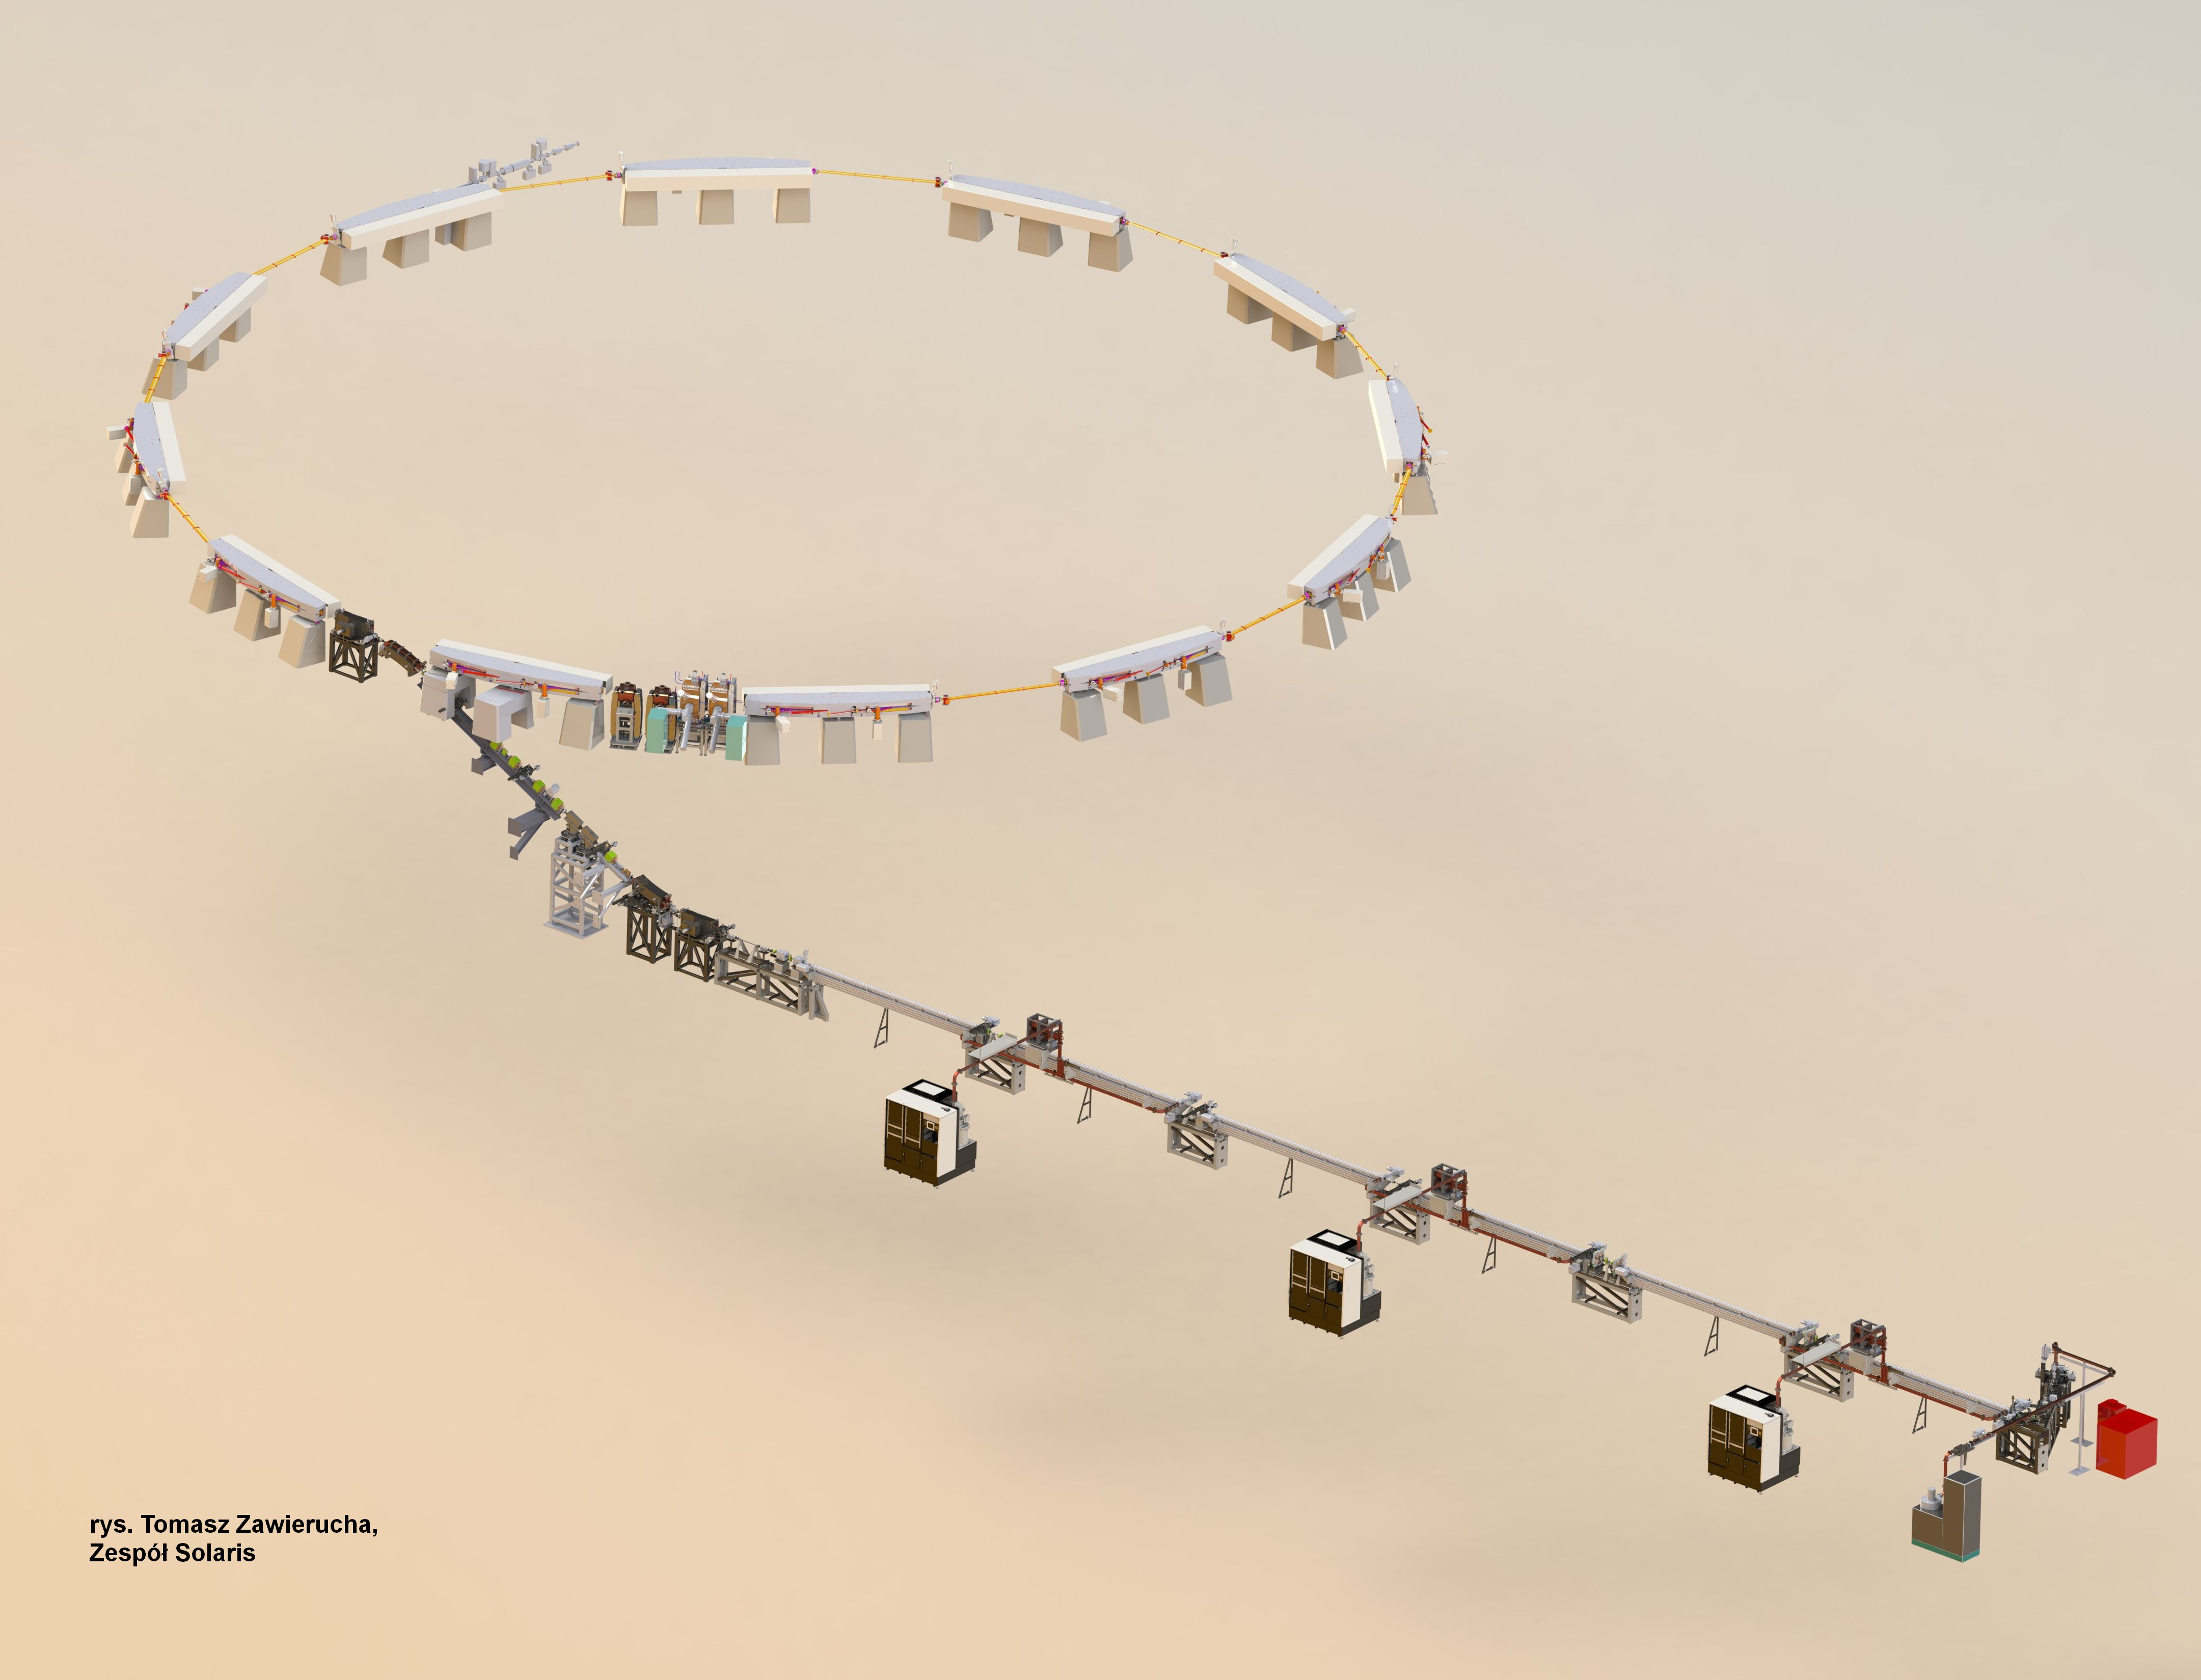
\includegraphics[width=0.9\linewidth]{Grafika/solarisMaszyna}
		\caption{Schemat synchrotronu znajdującego się w Solarisie. Źródło: \cite{synchrotron_uj_edu}}
		\label{fig:schematSynchrotronu}
	\end{figure}
	
	
	\hspace{2em} Promieniowanie synchrotronowe, jakie emituje pierścień akumulacyjny badane jest w specjalnych liniach badawczych, w skład których wchodzą skomplikowane mechanizmy składajace się z różnego rodzaju przesłon, zwierciadeł, pryzmatów itp. Każdy z tych elementów sterowany jest silnikiem krokowym, stąd istnieje konieczność synchronicznej pracy tych silników. Schemat lini badawczej przestawiono na rys. (\ref{fig:schematliniBadawczej})
	\newline
	\newline
	\newline
	
	\begin{figure}[ht]
		\centering
		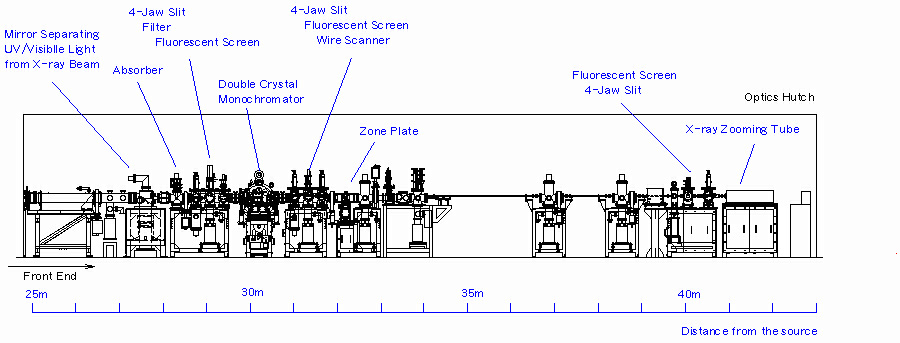
\includegraphics[width=0.9\linewidth]{Grafika/liniaBadawcza}
		\caption{Schemat lini badawczej. Źródło: \cite{web:exp_line}.}
		\label{fig:schematliniBadawczej}
	\end{figure}
	
\subsection{Systemy SCADA}
	
	\hspace{2em}Systemy SCADA (ang. Supervisory control and data acquisition) to system do zdalnego monitorowania i sterowania procesem techologicznym. Głównymi funkcjami systemów SCADA są:
	
	\begin{itemize}
		\item zbieranie aktualnych danych (pomiarów)
		\item wizualizacja danych
		\item sterowanie procesem
		\item alarmowanie
		\item archiwizacja danych	
	\end{itemize}
	
	\hspace{2em}Systemy te dają możliwość współpracy ze sterownikami PLC, regulatorami mikroprocesorowymi i innymi urządzeniami. Pozwalają na realizację zdecentralizowanych systemów automatyki przemysłowej. Systemy SCADA pozwalają na uzyskanie szybkiego wglądu w faktyczny stan urządzeń produkcyjnych i wykonawczych. Są one doskonałym sposobem nie tylko na zamianę języka maszyn na język ludzi, ale także umożliwiają szybką lokalizację alarmów, podstawowe logowanie danych czy też automatyczną reakcję na określone sygnały pochodzące z urządzeń. System SCADA w warstwie graficznej odpowiada za jednoznaczne zaprezentowanie dynamicznie zmieniającej się informacji. Jednocześnie zdefiniowane przez użytkownika algorytmy logiczne przyspieszają i wspomagają operatora w jego pracy. System SCADA jest także podstawowym źródłem danych dla systemów nadrzędnych i przemysłowych baz danych.
	

